\documentclass[10pt, a4paper]{article}
\usepackage[T1]{fontenc}
\usepackage[utf8]{inputenc}
\usepackage[swedish]{babel}
\usepackage{ifpdf}
\usepackage[parfill]{parskip}
\usepackage{graphicx}

\title{EIT060 2nd Project}
\date{}
\author{
	\begin{tabular}{l l}
		Tommy Olofsson & \texttt{<ada09tol@student.lu.se>}\\
		Erik Westrup & \texttt{<ada09ewe@student.lu.se>}\\
		Gustaf Waldermarson & \texttt{<ada09gwa@student.lu.se>}\\
		Erik Jansson & \texttt{<ada09eja@student.lu.se>}
	\end{tabular}
}

\begin{document}

\begin{titlepage}
\maketitle
\begin{center}
\end{center}

\thispagestyle{empty}
\end{titlepage}
\setcounter{page}{2}
% content
\section{System Description}
The system should handle medical records for patients. It consists of multiple entities including patients, doctors, and agencies. % oxford comma ftw

The entities are as follows:
\begin{itemize}
\item Patient: A patient can have one or more records in the system and he will at all time have read access to them. He will have to use private and public keys and a software client to obtain them from a server. 
\item Doctor: A doctor works at a department and will have read, write and create access for records to all patients registered to him. Also all records associated with the same department will be readable.
\item Nurse: A nurse works under a department will have read and write access to records for records to all patients registered to him/her. Also all records associated with the same department will be readable to the nurse.
\item Medical record: A medical record is stored on a server. Each record is associated with one patient, one doctor, one nurse and one department.
\item Agency: An agency will have the ability to list, read and delete records at will.
\item Certificate Authority: All certificates are signed by a root CA and every entity trusts this CA, this CA is separate from the hospital.
\item The server sits in a locked room and it accessible only by trusted technicians. Is has an audit log containing all access to the patient records.
\end{itemize}

\section{Setup Process}
The first step in setting the system up (apart from server installation and hardware distribution) is to generate a key pair and from this a Certificate Signing Request (CSR) for the public key. The CSR is transfered over sneakernet to the CA where it is signed and taken back and stored. 

A patient will need to obtain the system independent Java-client software from the ``socialstyrelsen'' office. They will there get their certificate signed. This certificate stored in the users private and protected keystore. They will also get a truststore with the certificate of the CA. All this will be put on a read only media (e.g. compact disc) that the patient can carry home and put his/her computer.

In a further extension of this system, it should be possible to add new doctors and nurses. This, however, is out of the scope of this project.

\section{Authentication}
The system will use two-factor authentication to connect to the server. The first factor is a password the user has to enter to get the unlock the keystore and one password for the truststore. These certificates are then used as the second factor, and are used to authenticate the user to the server. The certificates are valid for one year the password policy requres 13 characters from the set of upper and lower case letters and numbers. The password is also choosen in such a way that it cannot be cracked using a dictionary attack. These requirements were chosen to make sure that the password would not be cracked with a brute-force search within the timeframe of a single year.

\section{Protocol}
\subsection{Read}
Read will return the requested record if the user is \ldots
\begin{itemize}
	\item Patient: A patient can read a specific record with this command by supplying a record id. Returns the record or error if not found.
	\item Doctor, Nurse, Agency: A parameter specifying which record to obtain is needed. Returns the record or an error if not found or access denied.
\end{itemize}

\subsection{Append}
\begin{itemize}
\item Patient: Access always denied with a message "You shall not pass!".
\item Doctor, Nurse: Two parameters with record id and text to append is submitted. Responds with success or denied. Note that a doctor could mistype the id and accidentally write to another patients journal. A final product would include a GUI which would eliminate this problem.
\item Agency: Access always denied with a message "You shall not pass!".
\end{itemize}

\subsection{Create}
Creates a new record for a patient.
\begin{itemize}
\item Patient: Access always denied with a message "You shall not pass!".
\item Doctor: Parameters are patient id, nurse id.
\item Nurse: Access always denied with a message "You shall not pass!".
\item Agency: Access always denied with a message "You shall not pass!".
\end{itemize}

\subsection{Delete}
Removes a particular record.
\begin{itemize}
\item Patient: Access always denied with a message "You shall not pass!".
\item Doctor: Access always denied with a message "You shall not pass!".
\item Nurse: Access always denied with a message "You shall not pass!".
\item Agency: Parameter with journal id to delete. Returns success.
\end{itemize}

\subsection{List}
\begin{itemize}
\item Patient: If called by a patient with no parameters, it will list all records pertaining to the patient.
\item Doctor, Nurse, Agency: If called by a doctor or a nurse with a patient id as a parameter, it will list all records belonging to that patient. If no parameter is specified, an error is displayed.
\end{itemize}

\subsection{Implementation}
In the name of simplicity and convenience for the implementators no fancy protocol is used. The same commands describes above are sent directly to the server from the client with a message length prepended. The server can answer with two commands: error and result. The first is sent when a requested action is denied or failed and a text message is included. If the requested was successful a result is sent with the result text included.
\section{Public-key Infrastructure}
\label{sec+pki}

Asymmetric keys is a way of letting two parties communicate securely without having a shared secret (like in symmetric encryption) but instead by both having a private/public key pair. The public keys are shared and messages are encrypted with them. Only the holder of the corresponding private pair can decrypt it. The only problem with this is that you don't know who's public key you have meaning you could have a perfectly secure connection to a fraudster! One way to solve this is to let a Trusted Third Party verify the public key and map it to a real identity. There is an hierarchical order where the \emph{Root Certificate Authorities} are on the top. 

When someone want to prove the key-identity connection to someone they can generate a certificate request and let a CA sign it with its private key. The signed certificate can then be shared to others publicly. Other users who trust the same CA can then verify this signing by decrypting the certificate with the CAs public key. The signing can possibly be applied in several steps creating a certificate chain. To verify a certificate chain you have to follow it up from bottom to top and verify each signing. If you find a CA in the chain that you trust you can also trust the certificate from the unknown person.

One problem for the user is to get the root CAs. Typically they are included in operating systems or in web browsers. The user thus have to trust the judgment of the distributer of these systems that they use. Another problem is when security is breached, e.g. when a CAs private signing key is lost to a fraudster. Then the fraudster can sign certificates in the name of the attacked CA. A proposed but not working solution is to regularly publish a \emph{Certificate Revocation List} of certificates that no longer should be trusted. The users is supposed to check these lists regularly but in practice there is no standardized way of doing this.

One alternative and decentralized approach which is not based on TTPs is \emph{Web of Trust}. This is instead based on a system of voting where the identity of a public key is strengthened by the fact that many others trust this connection.

\footnote{Computer Security 3ed, Dieter Gollman, Wiley, page 288-293}

\section{SSL/TLS}
\label{sec+tls}
In our system we are using \emph{SSL/TLS}\footnote{Secure Socket Layer/Transport Layer Security}-technology for authentication and establishment of a secure connection between the communicating parties. SSL was developed as a client-server protocol to be used to provide a secure byte stream on top of transport layer in the TCP/IP-stack for application protocols like http and email. Work on SSL started in the mid 90s by Netscape and was eventually adopted as a standard. SSL has lately been superseded by TLS. However the last version of SSL, 3.0, only differs slightly from TLS 1.0 and thus you often refer to the technology as SSL/TLS. We will here refer to TLS as it is the new  and recommended protocol to use. By using TLS in our program we will achieve mutual authentication between server and client, message confidentiality and integrity. The mutual two-way authentication is optional but since we are using it it will be described below.


\subsection{Pre-handshake}
It is assumed that both the server and the client have generated a public/private key pair and have a CSR signed by a CA according to section \ref{sec+pki}. It is essential that both sides trust at least one CA in the certificate chain of the other party -- otherwise they will not be able to trust each other. In our case a common root CA is used for certificate signing.

\subsection{Handshake}
Note that the order used when describing the handshake is logical and not the actual order the different parts are sent over the wire. Many of these steps are sent all at once. The first part in the handshake is that the client initiates the communication by sending a \emph{ClientHello} to the server containing a random number (used later) and a list of supported cipher suits ranked in the order of the clients preference. A cipher suite is a text string specifying a set of parameters in the form \emph{<ssl/tls>\_<keyexchange>\_WITH\_<encyption-type>\_<enc-key-size>\_<hmac>}. For example \emph{TLS\_RSA\_WITH\_RC4\_128\_SHA} means that to use Transport Layer Protocol with RSA authentication and message encryption with RC4 stream cipher with 128 bit keys and that the hashed message autentication to be used is Secure Hash Algorithm. The client can also optionally specify a compression algorithm to use in this message. The server responds with a \emph{ServerHello} including a random number and a chosen cipher suite that is the best match from the client and the servers preferences. When we tested our program the client and server agreeded on using \emph{TLS\_DHE\_DSS\_WITH\_AES\_128\_CBC\_SHA} which uses Ephemeral Diffie-Hellman for key exchange, and AES with 128 bit sized keys and Chain Block Cipher mode for message encryption and SHA1 as hash algorithm. We will use this cipher suite the rest of the TLS discussion here.

Optionally the server now (as in our program) wants to identify the client to be able to correctly authenticate it so it can use the provided services. Optionally (and most often) the client wants to  identify the server so it knows from whom he is about to request services from. It might be the first time they communicate so no previous shared secret between them exists. This is solved by letting a trusted third party\footnote{TTP} verify the identity of one part. Thus they now have to to exchange certificates. The server then send its \emph{certificate} or the whole certificate chain to the client. If it wants to identity the client it also send a \emph{certificate request}. The following message is \emph{SeverHelloDone} indicating the end of this phase from the servers side.  The client verifies the servers certificate if one was recieved. If the server requested so, the client send its certificate or the whole certificate chain to the server who then verifies it.

Next the client will send \emph{ClientKeyExchange} which is dependent on the previously chosen key exchange algorithm. In our case Ephemeral Diffie-Hellman (DHE) is used. They now agree on a modulus and a generator. Both sides raises the generator in the power of a generated random number and sends it to the other side. By combining these the now share a secret depending on the discrete logarithm problem. The only problem is here the MITM\footnote{Man in the Middle.}-attack. This is solved in DHE by signing the sent values  with their respecive private keys.

The client now send \emph{ChangeCipherSpec} and \emph{Finished} meaning that from now on all communication will be encrypted using the now shared secret. The server answers with the same sequence.

\begin{figure}[hbt]
  \begin{center}
    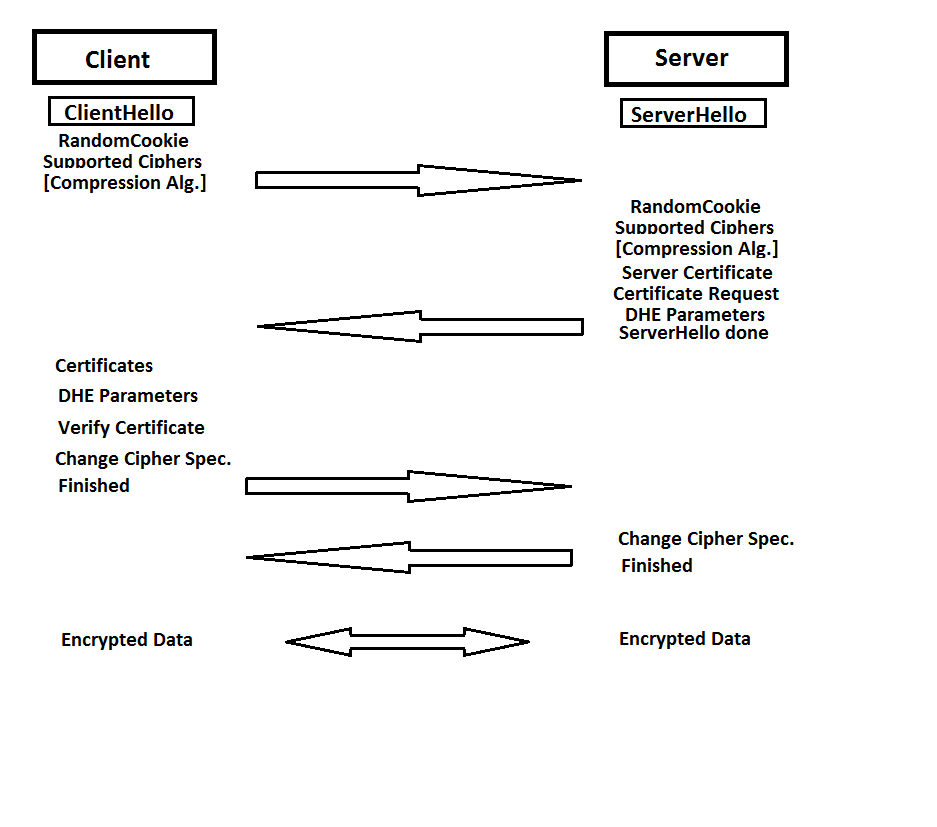
\includegraphics[scale=0.6]{protocol.png}
  \end{center}
\end{figure}

\subsection{Communication}
Now both parties have agreed upon how to communicate and with what keys. The messages is encrypted using the specified block or stream cipher and the HMAC is sent, allowing the receiver to verify the integrity of the message.

\subsection{Teardown}
Both sides must send a \emph{Close Message} to terminate the session.


\footnote{Computer Security 3ed, Dieter Gollman, Wiley, page 310-314}
\footnote{Java\textregistered Secure Socket Extension (JSSE) Reference Guide, accessed 2012-02-09, http://docs.oracle.com/javase/6/docs/technotes/guides/security/jsse/JSSERefGuide.html}


\section{Security Evaluation}
A list of attacks we are safe against:
\begin{description}
\item[Man-in-the-middle] Defending against a man-in-the-middle attack is hard without using a second, secure channel for verification. However, by using SSL-connections and certificates signed by a common certificate authority, this attack is avoided. An eavesdropper, from here on called Eve, would need to trick the certificate authority into signing her certificate with the servers name on it. This should not be possible since the CA checks identities of all certificates it signs.
\item[Eavesdropping] This attack is simply averted by using the SSL protocol, see Section~\ref{sec+tls} for a more detailed explanation of SSL.
\item[Fake certificates] Since we're using a single certificate authority which signs all the certificates, no certificates signed by anyone else than our CA is accepted. Thus, this attack vector is eliminated.
\end{description}

A list of attacks we are vulnerable against:
\begin{description}
\item[Spoofed Client] If an attacker writes a fake client and tricks a user into using it as the real one. We cannot defend the users against that. The most severe thing the malicious attacker can do in this scenario is to steal all health information the user accesses. Unfortunately, the only ways to defend against this is to make sure that the correct client has been downloaded by visiting the hospital website using an SSL-connection or been obtained through some other secure way.

Some user education would be required to make sure they always download the software from the hospital's secure web server which authenticates itself with an SSL-certificate signed by a certificate authority which is trusted by all browsers, e.g.~VeriSign or DigiCert. This is needed to avoid the possibility that the user can accidentally receive a malicious client which steals patient information.

\item[Compromised Keystores]The human factor is hard to take into account, a user will always do things you have not predicted with the software. For example, our implementation cannot protect against the user choosing a short and weak password which are prone to be broken since the password is handled by the Java keytool utility.

In a real system, the client software would put some requirements on the password, e.g.~alphanumerical passwords of length 10 or more. This would give $(26*2 + 10)^{10} \approx 8.39\cdot 10^{17}$ possible combination of passwords which would take approximately 2 years and 7 months to enumerate at 10 billion passwords per second\footnote{http://www.wolframalpha.com/input/?i=\%2826*2\%2B10\%29\%5E10+\%2F+10\%5E10+s}. Since we will have an expiration time of one year, this seems sufficient protection against weak passwords.

There is always the possibility that an attacker will have access to a super computer capable of cracking passwords at a \emph{significantly} higher rate than usual. This scenario is not easy to defend against. The only solution is to use an algorithm that, like bcrypt, can be made arbitrarty slow. This would not have any relevant inpact on legitimate use, seeing as there is just the one login at launch. The attacker on the other hand would undoubtably be slowed down considerably. However, using keytool, this is not an option since the keytool utility does not allow a choice of encryption algorithms when encrypting a keystore.
% TODO med vilken dator skulle det ta den tiden?

With the keystore password the attacker would have free access to a user's certificates. These can later be used by the attacker to authenticate himself/herself with the server.

\end{description}


\end{document}
